\documentclass{article}
\usepackage[utf8]{inputenc}
\usepackage{graphicx}
\usepackage[colorlinks=true]{hyperref}
\newcommand\tab[1][1cm]{\hspace*{#1}}


\title{CS 155 Group Project 3 Report}
\author{Derek Ing, Daniel Li, Joon Young Park, Hernan Caceres}
\date{March 2022}

\begin{document}

\maketitle

\section{Overview}
Using 22 late hours
\begin{enumerate}
    \item \textbf{Group members}:
    \vspace{2mm} 
    
    Hernan Caceres, Daniel Li, Derek Ing, Joon Young Park
    
    \item \textbf{Piazza Link}:
    \vspace{1.5mm} 
    
    \href{https://piazza.com/class/kxhtyed0nmh2s?cid=527}{ 
Click here.} 
    
    \item \textbf{Division of Labor}:
    \vspace{1.5mm} 
    
    \begin{enumerate}

        \item Derek Ing: Pre-processing, training, and poem generation for RNN
        
        \item Daniel Li: Pre-processing and poem generation for HMM. 
        
        \item Joon Young Park: Visualizations and implemented rhyming in HMM
        
        \item Hernan Caceres: 
        Preprocessing, implemented additional goals for HMM
    \end{enumerate}
\end{enumerate}

\newpage

\section{Pre-processing}

For the HMM, we did very little preprocessing. We simply took the text of Shakespeare and split it into words. We removed all capitalization and punctuation from the words before our generate emission function. After the generation of the function, capitalization was reintroduced to the start of each line as well as the word "I".\\
\\
For the RNN model, the pre-processing was slightly different because we build a character-based model. Similar to the HMM, we build a mapping of all unique characters to indices. However, we also include spaces, newline characters, and all punctuation so that the model can learn to put spaces between words and separate lines with newline characters. We initially did not include newline characters, spaces, or punctuation, but the generated poem was just a long sequence of letters. Thus, we included spaces, punctuation, and new line character. The poem generation seed given in the project also includes a question mark. In addition, in the poems, each line also usually ends with a punctuation mark. We also decided to make all alphabet letters lower case. 

\section{Unsupervised Learning}
We used the Baum-Welch algorithm implemented in HW6 to create our HMM for poem generation, with no other packages. We chose the number of hidden states simply based on the structure of the poem produced by the hidden states. With too few hidden states, the poem became incoherent, with what seemed to be completely random words generated. However, with too many hidden states, the poem becomes more populated with conjunctions and pronouns, rather than other words. We ended up settling on 16 hidden states, which seemed to provide a healthy balance between the incoherence and the excessive pronouns/conjunctions. We did not use any additional packages that weren't included in the original HW6 code.
\newpage
\section{Poem Generation: Hidden Markov Models}

\href{https://colab.research.google.com/drive/1l25ou9yO_X3g2_WjsuIXAGUL_YcAR7yZ?usp=sharing}{Colab Link}\\

The 14 line sonnet was generated using a HMM model with unsupervised training. Our algorithm involved modifying the generate emission process. We first start by choosing a random state. We then sample the next observation to find the next word. If the next word does not meet the syllable requirements, we repeat this process until a word that meets the syllable requirements is found. We store this emission and then move to sample the next state. 
\newline

The poem we generated is as follows:
\newline

Love more to presentst thou needs thy painted \newline
Subject for me be mock dost take virtue \newline
Main the shade and the sees have bears where I \newline
O all you roses can abundant of \newline
Thou in near thou for thy he as thing if \newline
Divide turns but that beautys sleep if breath \newline
Bear strength those far the beauty thoughts eat they \newline
Him my flesh mark then shamed sharpened three you \newline
And the scythe and with grace I swear for in \newline
All the thought of and truetelling to and \newline
That reckoned of sins found for thou tears thy \newline
Which of sorrow to her ay whence for not \newline
We worthy single powers pass whoever \newline
Seeming eves cold woe shade approve self I \newline

With regard to rhyme, using this approach did nor result in rhyme (we added further modifications that do end up yielding a sonnet with a rhyme scheme later on.) To analyze rhythm, we look for iambic pentameter in the lines. Since our algorithm ensures syllable count constraints, each line of the poem is indeed ten syllables. With regard to the unstressed stressed repetition in each line, although it is not perfect, there are multiple lines that adhere to the unstressed stressed pattern throughout the entire line (the first two lines follow this pattern). However, there are some lines in which the unstressed stressed pattern is lost (in line 3, the word triplet “sees have bears” arguably have 3 stressed syllables consecutively. Even if poetry is meant to be abstract, our poem as a whole makes little sense. On a line by line basis, many of the lines resemble lines of a Shakespearean sonnet and maintain Shakespeares voice, such as lines 6 and 11. However, there are lines that do not make sense in essentially any context, such as line 5. And even though some lines standalone resemble Shakespeare, at the quatrain and whole poem level, the lines do not have any direction or relation with each other. For this reason, the sonnet also seems to lack a volta. When we tested the effect of the number of hidden states included in the model, it was found that as the number of hidden states increases, the more conjunctions and pronouns are used throughout the sonnet. As mentioned, the unstressed stressed pattern is decently captured by the model. Our intuition as to how the HMM was able to capture this quality is that it detected the pattern, and when a stressed sound was required, it used a word that starts with t, as the sound produced by t is very stressed. This is supported by the high count of words that start with t in the sonnet. 


\newpage
\section{Poem Generation: Recurrent Neural Network}
\href{https://colab.research.google.com/drive/10wlawrgl-Orz6RBJFQbeqVHr1Sl3VOs1?usp=sharing}{Colab Link}\\

We built a character-based LSTM RNN model, we used PyTorch's implementation. The model we implemented has a single layer of 200 LSTM units, using torch.nn's LSTM module, followed by a fully connected linear layer, and lastly a log softmax nonlinearity, similar to the model in the tutorial provided in the project specifications. We initially tried using a softmax nonlinearity, but we found that the model produced higher quality poems when training with a log softmax nonlinearity. To make predictions, we take the exponent of the log softmax output. The LSTM allows the RNN model to pass on relevant information and forget information that is not relevant. Thus, the RNN can keep track of important information from previous inputs to make a prediction on the current input sequence. The output is then looped back into the network. Thus, the RNN can learn sequences of characters, such as words, or even when to add spaces or punctuation or make a new line.\\

Training inputs to the RNN were sequences of 40 characters, and the target output was the character occuring right after the last character of the input sequence. To obtain the sequences, we took all possible subsequences of 40 characters starting every 10th character to speed up training. We also converted each character into a one-hot-encoded vector, using a mapping of unique characters to unique indexes. Thus, each vector has all 0 entries except for a 1 entry on the index corresponding to the character provided by the mapping.\\ 

To train the RNN, we used the RMSprop optimizer provided by torch.optim, and trained in batches of 512 sequences. We trained the RNN to minimize categorical cross-entropy loss, provided by Pytorch. We tuned the learning rate and number of epochs trained. We ended up with a learning rate of $0.005$ and trained over 100 epochs. We discovered that during training, the loss decreases significantly at first, but when we expect the loss to converge, the loss occasionally significantly spikes up and decreases again. Thus, we also chose to use an early stopping condition, which was to stop training if the total loss across all batches was $< 0.5$ (the initial total loss was $\approx 70$). \\

Finally, we generate poems by sampling 520 characters (assuming each line is around 40 characters) from the exponent of the log softmax output of the model with the initial seed: "shall i compare thee to a summer's day?$\backslash$n".\\

Temperature = 0.25:\\
shall i compare thee to a summer's day?\\
to somed tor my sifersing of sullt,\\
and they how,\\
thy seall to spert dows sould,\\
the will buswing all awdith tn me,\\
rof dotheried beauty heartere fir hearte,\\
whereive woush the enemy sand,\\
in in they ase my self,\\
and tele shoug,\\
tor in tell spow that thou this this be: on nore,\\
ould to his res shate swealt thou wort, and iy the lievs prostind an with telu porant hives mine allave,\\
and noth can yot she tid, and thee he with thy sell thou art not but e dofarin,\\
ou parth the reauty love wor de,\\
oulfane in in thee then\\

Temperature = 0.75:\\
shall i compare thee to a summer's day?\\
to shough thise when toug trie,\\
worl, thou all, ne rape thou gitty,\\
and her the lood,\\
the bein i some,\\
and all mane arfimite,\\
whe of thy sealten whough to shie werced wor the liges loves ure troe,\\
our pe thin they bugh dove whe buad\\
to shinds i four!st me tham min boastrs chy add my spen bot share sive,\\
whish hat ing more,\\
worsspnot that i soou porthe,\\
oven they llow ng preet of self,\\
inen seenks whid is ins mane thou art not make tovere,\\
ave tour of thos thy hemose to be perre,\\
wothy ingresteds primely of reare,\\
b\\


Temperature = 1.5:\\
shall i compare thee to a summer's day?\\
eourd in mines buted which cony erth,\\
the bearyel kerime,\\
the earp, wosthe ealt insimstle,\\
ther fand:\\
mencill toujh me erow's they grod:\\
rord tirs i pore- op forn bot shall heveewberte frommtht\\ ondwent'inc iulbrppeine,\\
thou may:\\
rory for heapleth freidnd ihend imen\\
willou, which in letes mibe it,\\
and coun ay )\\
ar's son tho ,\\
oows ,or yot me ressint:\\
ayn.\\
the fai frean all write,\\
but that shougn sing mises re,\\
all vencaye whereforr prrieid,\\
or'mlsosd hir be tho sweed tom me,\\
onet beawgy tiver's forst do wiles nee yo\\


We see that temperature has a significant impact on the poems generated by the model. The poem generated with the lowest temperature looks most like a Shakespearean sonnet. The poem generated with temperature $=0.25$ has several English words and some sentence structure in the lines. On the other hand, the poem generated with temperature $=1.5$ has very little real English words. However, we do wee more varied punctuation and word length with higher temperature. The poem generated with temperature $=0.75$ is similar to the first poem in line length and structure, but there are less English words. The model can also learn some line structure. For example, we see the model learns to put spaces between words and some punctuation, as well as putting new line characters after each line. The model does not learn the sonnet structure too well. The number of lines produced were around 15-16, which is slightly more than the 14 lines in a Shakespearean sonnet. In addition, the length and number of syllables in each line is quite inconsistent. However, there are no other features that resemble a Shakespearean sonnet.\\

Compared to the HMM, the LSTM generates much lower quality poems. The LSTM also takes a longer time to generate a poem (1 minute compared to a couple seconds). If we had more training data and trained the LSTM for longer, the LSTM could produce poems of similar quality to the HMM.
\newpage


\section{Additional Goals}
\href{https://colab.research.google.com/drive/1A5OMDkiRWHaEmUsSPmJMswrTzo2o-q64?usp=sharing}{Colab Link}\\

On top of the original generated sonnet, we generated sonnets with rhyme: \\
\\
See I more ladies against contain thence \\
Buried torment love deeds he his snow scorn \\
A four confound name hold intelligence \\ 
Thy with labouring majesty he outworn \\
Pure thy in to tresses in all perish \\
Same which some what beguiled to carcanet \\
Fortune monuments is I and cherish \\ 
Love the and lease thinks stoln added my set \\
Review how and the youth lovers exceeds \\ 
Next thee becomes her shine in wet doth sight \\ 
In sickness own with with in kill strong deeds \\
Thy to grow points true feedst will thy of write \\
\tab That hid white hath bright will for limbs exceeds \\
\tab Powerful to leave correspondence bids deeds \\

In our generation of the rhyming sonnet, we ran into issues adding the rhyming word to the end of the sentence which would fit the number of syllables necessary for the traditional 10 syllable line. Eventually, we proceeded by adding the word to the beginning of the states through the generate emission function and generating words after that. We would then reverse the sentence produced by the generate emission function, allowing the rhyming word to be put at the end of the sentence as well as meeting the required number of syllables. We think that the addition of the rhyming elevated the poem to be more like the original Shakespearean text. We don't really see any diminishing in the quality or creativity of the sonnet.

\newpage

\section{Visualization \& Interpretation}
Similar to what we have done on Set 6, we created a visualization for representing sparsity of transition and observation matrix. For further analysis, we have printed out the top 10 words that associate with the hidden state with the common feature among these groups for 5 different hidden states. At the next page we have included visualization of sparsity of transition and observation matrix. 

\begin{figure}[htp]
        \centering
        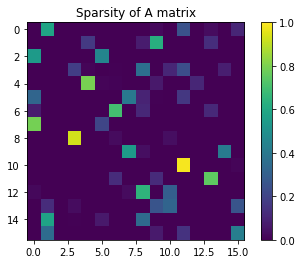
\includegraphics[width=0.8\textwidth]{transition.png}
        \label{fig:figure1}

        \centering
        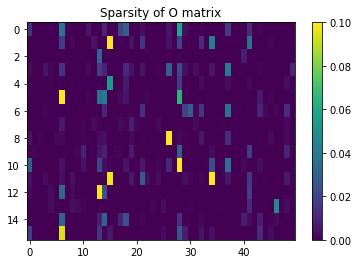
\includegraphics[width=0.8\textwidth]{observation.png}
        \label{fig:figure1}
\end{figure}


Below is the list of top 10 words associate with the respective hidden state for 5 different hidden states: \newline

State 1: ['love', 'doth', 'beauty', 'heart', 'world', 'thou', 'sweet', 'fair', 'life', 'self'] $\rightarrow$ love related words and possessive words \\
State 3: ['thou', 'thy', 'yet', 'will', 'art', 'time', 'may', 'must', 'show', 'love']$\rightarrow$ modal verbs and possessive words\\
State 4: ['night', 'love', 'poor', 'loving', 'pleasure', 'friend', 'soul', 'one', 'lovely', 'best'] $\rightarrow$ adjectives and love-related nouns\\
State 10: ['thy', 'every', 'make', 'time', 'show', 'love', 'mine', 'thee', 'give', 'one'] $\rightarrow$ possessive words \\
State 11: ['love', 'self', 'heart', 'thee', 'eye', 'will', 'mind', 'beauty', 'verse', 'sweet'] $\rightarrow$ beauty/love related words\\


Note that at the end of the list for each state, we have identified the common features among these groups. First of all, based on the visualization below, we can clearly see that both the transition and observation matrix are both pretty equally sparse. The sparsity for A matrix would mean that for each state, there are limited number of states such that the HMM model could transition into. For example, we can see that the transition from state 10 would only lead to one state, which is state 11, as it can be clearly seen from the visualization where when the initial state is 10, the entire row is dark except one slot where final state is equal to 11 (colored as yellow). This makes sense since state 10 words are mostly associated with "possessive words", while state 11 words seem to be associated with beauty and love. We know that Shakespeare enjoys writing about the theme of love in sonnets, such as courtly love, unrequited love, compassionate love, etc. Considering that the love is a recurring theme in his sonnets, we can infer that the transition from "possessive" words to love-related words would happen very frequently (e.g. thy beauty, make love, etc.). 

In the case of O (observation) matrix, the sparsity here would mean that there are only few observations that can be made given some state. We can see that there are several transitions where its probability is pretty high, which makes sense, as these usually correspond to frequently occurring words. Some of these would include articles, such as "a", "the", as well as transition words (e.g. "and", "but") and Shakespearean words (e.g. "thee", "thy", etc.).

\newpage



\section{Extra Credit} 
\href{https://colab.research.google.com/drive/1l25ou9yO_X3g2_WjsuIXAGUL_YcAR7yZ?usp=sharing}{Colab Link}\\


We implemented generating other poetic forms (haiku): \\
\\ Save niggard add mind \\
All for but stands in thee of \\ 
Why that outbraves thy \\
\\
We ran into very few issues regarding the generation of the sonnet. Rather than the traditional 10 syllables per line, we simply had to change this number in the sentence generation function to match the number of syllables for each line in the sonnet. The haiku seems to hold with consistent quality/creativity as our previously generated sonnet. \\ 
\\
We also incorporated additional texts into our model. Here is a sonnet generated with the additional texts: \\
\\ Use yet time others where victor in thee \\
To that love pace and that clean returned with\\
Me bevel thy is told fall pleasure sun\\
Used that most not stronger that all others\\
What beauty surmise a heat doth though shows\\
Should a full millions to may it old will\\
And beloved of me or thrust so mock all\\
Dulness my thee shown times left your thee where\\
But with survive not thou to rightly fruit\\
But to I before my since bark skill best\\
Tonguetied graces bring my wound excuse a\\
And with phoenix I fair choose solemn same\\
\tab Even proved true wrongs a by grace that had my\\
\tab That thee in one he again and they self\\
\\
We can see that our sonnet generated with the multiple texts seems to have more variety in its vernacular. We ran into a slight issue still attempting to assert that the number of syllables in each line was equivalent to 10. This issue was dealt with by simply assuming that the number of syllables in a word was equivalent to the length of the word divided by 3, as the average number of letters per syllable is 3. Again, there seems to be a consistency in the quality/creativity of the originally generated sonnet.



\end{document}
